\documentclass{article}
\usepackage[utf8]{inputenc}
\usepackage[spanish,es-tabla]{babel}
\usepackage{amsmath,amsthm}
\usepackage{xfrac}
\usepackage{graphicx, float}
\usepackage{adjustbox} % Permite detallar el tamaño de las tablas
\usepackage{amssymb}
\usepackage{enumitem}
\usepackage{wrapfig}
\usepackage{import}
\usepackage[dvipsnames]{xcolor}
\usepackage[spanish,onelanguage]{algorithm2e} % Pseudocódigo
\usepackage[colorlinks,linkcolor=BrickRed,urlcolor=Blue]{hyperref} % URLs, referencias a tablas
\usepackage{mathpazo} % Palatino font
\usepackage{multirow} % Múltiples filas por celda

\DeclareMathOperator*{\argmin}{argmin}

% Entorno para controlar el espacio antes y después de un algoritmo
\newenvironment{algo}{
	\vspace*{0.5cm}
	\begin{algorithm}[H]}{
	\end{algorithm}
	\vspace*{0.5cm}
}
\SetKwBlock{Repeatn}{repetir}{}

% ///////////////////////////////////////////////////////////////////////////////////////
% Se ha usado la plantilla https://www.latextemplates.com/template/academic-title-page
% Autoría de la plantilla
% WikiBooks (LaTeX - Title Creation) with modifications by:
% Vel (vel@latextemplates.com)
%
% Licencia de la plantilla:
% CC BY-NC-SA 3.0 (http://creativecommons.org/licenses/by-nc-sa/3.0/)
% ///////////////////////////////////////////////////////////////////////////////////////

\begin{document}

\begin{titlepage} % Suppresses displaying the page number on the title page and the subsequent page counts as page 1
	\newcommand{\HRule}{\rule{\linewidth}{0.5mm}} % Defines a new command for horizontal lines, change thickness here
	
	\center % Centre everything on the page
	
	%------------------------------------------------
	%	Headings
	%------------------------------------------------
	
	\textsc{\LARGE Universidad de Granada}\\[1.5cm] % Main heading such as the name of your university/college
	
	\textsc{Metaheurísticas}\\[0.3cm] % Major heading such as course name
	
	\textsc{Curso 2017-2018}\\[0.5cm] % Minor heading such as course title
	
	%------------------------------------------------
	%	Title
	%------------------------------------------------
	
	\HRule\\[0.4cm]
	{\huge\bfseries Práctica 3: Enfriamiento Simulado, Búsqueda Local Reiterada y Evolución Diferencial}\\[0.4cm] % Title of your document
	
	\HRule\\[1.5cm]
	
	\textsc{Aprendizaje de Pesos en Características}\\[0.5cm]
	
	\vfill

	\textsc{José Manuel Muñoz Fuentes}\\
	\input{DNI.txt}\\
	\texttt{jmlosvillares@correo.ugr.es}\\
	{\footnotesize\textsc{Grupo de prácticas 2 (martes 17:30 - 19:30)}}

	\vfill\vfill\vfill % Position the date 3/4 down the remaining page
	
	{\large\today} % Date, change the \today to a set date if you want to be precise

	\vfill\vfill
	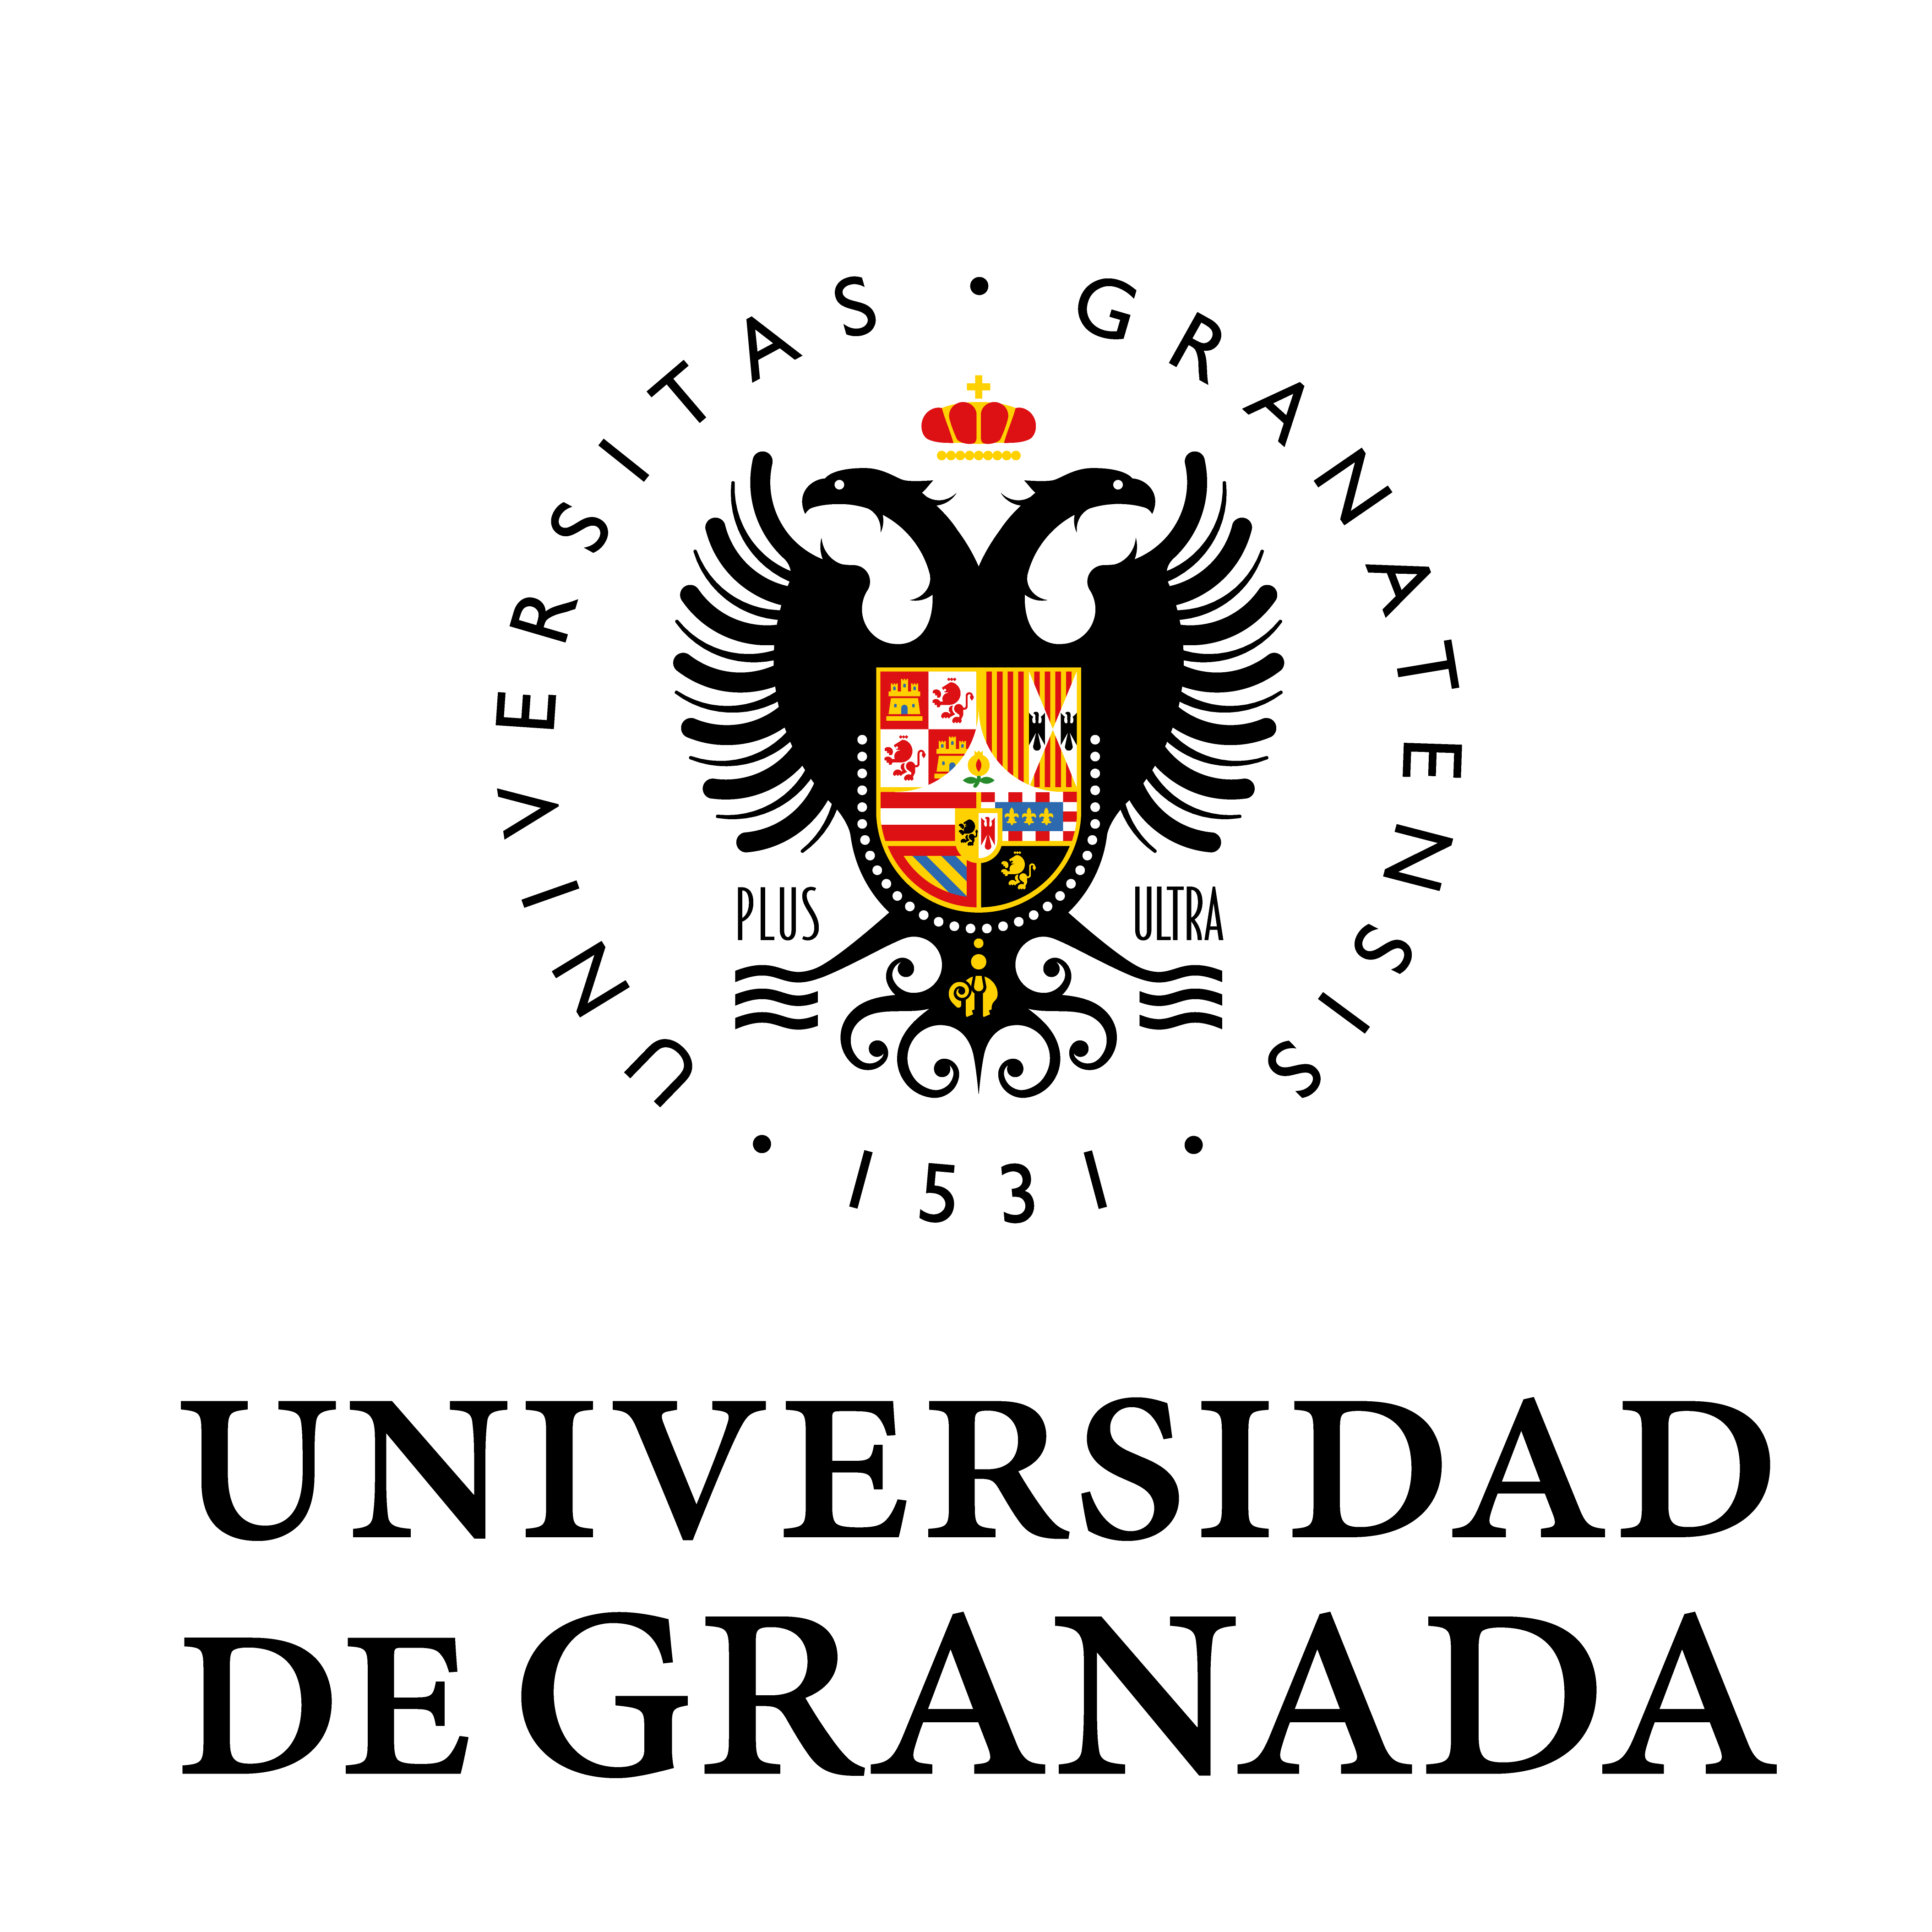
\includegraphics[width=0.2\textwidth]{ugr.png}\\[1cm] % Include a department/university logo - this will require the graphicx package
	
	%----------------------------------------------------------------------------------------
	
	\vfill % Push the date up 1/4 of the remaining page
	
\end{titlepage}
\tableofcontents

\section{Descripción del problema}

El aprendizaje automático supervisado contempla, entre otros problemas, la obtención de métodos de clasificación, los cuales tratan de asignar clases a datos a partir de una muestra de datos clasificados según un criterio a priori desconocido por la máquina. Uno de los algoritmos de clasificación más conocidos es la clasificación $k$-NN, en la que a cada dato se le asigna la clase más común de sus $k$ vecinos más \textit{cercanos}. Para ello se define una función que computa la distancia entre dos datos, que se representan como una tupla de valores numéricos o categóricos; se evalúa la distancia entre el dato a clasificar y todos los elementos de una muestra de entrenamiento y se asigna la categoría más frecuente en los $k$ datos de la muestra que están a menor distancia del dato. Una versión general del problema propuesto consistiría en obtener una función distancia que, al ser utilizada, permita elaborar un clasificador óptimo en cierto sentido. \\

Para las prácticas de esta asignatura se aplicarán las siguientes restricciones al problema general:
\begin{itemize}
  \item Se considera la clasificación $1$-NN, donde simplemente se asigna a cada dato la clase del dato a menor distancia de este (llamado su \textit{vecino más cercano}) en la muestra de entrenamiento.
  \item Se utilizará como espacio de posibles funciones distancia aquellas de la forma $\sqrt{\sum_i w_i (x_i - d_i)^2}$ donde $x_i$ y $d_i$ son la componente $i$-ésima de las tuplas que representan, respectivamente, un dato de la muestra de entrenamiento $\normalfont \textbf x$ y un dato a clasificar $\normalfont \textbf d$, y $w_i$ es el elemento $i$-ésimo de un conjunto de \textbf{pesos} expresados como números reales nulos o en el intervalo $[0.2,\ 1]$. No será necesario computar la raíz cuadrada debido a que esta operación es biyectiva y monótona para números reales no negativos ($a = b \Leftrightarrow \sqrt a = \sqrt b$ y $a < b \Leftrightarrow \sqrt a < \sqrt b$) y por ello no afecta al cálculo del vecino más cercano. Por esta restricción, el problema se reduce a encontrar (o aprender) un conjunto de pesos $\normalfont \textbf w$ que conlleve un clasificador óptimo.
  \item Se evaluará cada clasificador según su capacidad para etiquetar elementos correctamente, el número de características que no considere y el tiempo de ejecución del algoritmo que se había utilizado para obtener el clasificador. Por la condición anterior, esto equivale a que se evalúe cada conjunto de pesos por la tasa de clasificaciones correctas de su clasificador, su número de pesos nulos y el tiempo necesario para obtener tales pesos.
\end{itemize}

El objetivo de todas las prácticas de esta asignatura será desarrollar, implementar y comparar algoritmos que, a partir de unos datos, tratan de obtener pesos óptimos para las características de dichos datos según el criterio de evaluación especificado.



\section{Aspectos comunes a todos los algoritmos}

Las soluciones se representan como tuplas de pesos con tantas componentes como el número de características observadas en la muestra. Cada peso $w_i$ se almacena como un valor real en $[0,\,1]$, de forma que la distancia al cuadrado entre dos datos $\normalfont \textbf x$ y $\normalfont \textbf d$ se calculará como $\sum_i \delta(w_i)(x_i - d_i)^2$, donde $\delta(x) = 0$ si $x < 0.2$ y $\delta(x) = x$ en caso contrario. Así, los pesos menores que $0.2$ en una solución son considerados nulos en el cálculo de la distancia entre dos datos. \\

La función objetivo, que evalúa una solución o vector de pesos $\textbf w$ sobre un conjunto de entrenamiento o de test $T$, se describe a continuación.

\begin{algo}
	\KwIn{$\normalfont \textbf w = \{w_1,\ ...,\ w_N\}$ tupla de pesos, $T$ conjunto}
	\KwOut{Valoración de la solución}\BlankLine
	
	$V_1 := 0$\;
	$V_2 := 0$\;
	\ForAll{$\normalfont \textbf d \in T$} {
		$\normalfont \textbf x := nearest(\normalfont \textbf d, T \setminus \{ \normalfont \textbf d \}, \normalfont \textbf w)$\;
		\lIf{$clase(\normalfont \textbf x) = clase(\normalfont \textbf d)$}{
			$V_1 := V_1 + 1$
		}	
	}
	\ForAll{$i$ \textnormal{\textbf{desde}} $1$ \textnormal{\textbf{hasta}} $N$} {
		\lIf{$w_i < 0.2$}{
			$V_2 := V_2 + 1$
		}
	}
	\KwRet{$\displaystyle \frac {V_1} {|T|} + \frac {V_2} N$}
	\vspace{0.2cm}
	\caption{Función objetivo, donde $clase$ es una función que devuelve la clase de un dato (que es conocida porque $T$ es un conjunto de entrenamiento o de test) y \hyperref[nn]{$nearest$} es la función que encuentra el dato más cercano.}
\end{algo}

La obtención de una solución aleatoria se efectúa así:

\begin{algo}
	\label{random}
	\KwIn{$N$ número de componentes}
	\KwOut{$\normalfont \textbf w_r$ solución aleatoria}\BlankLine

	\ForAll{$i$ \textnormal{\textbf{desde}} $1$ \textnormal{\textbf{hasta}} $N$}{
		$(\normalfont \textbf w_r)_i := Uniforme(0,\, 1)$
	}
	\KwRet{$\normalfont \textbf w_r / \max_{i = \{ 1,\ ...,\ N \}} (\normalfont \textbf w_r)_i$}
	\vspace{0.2cm}
	\caption{Algoritmo de obtención de una solución aleatoria de $N$ componentes. $Uniforme(0,\, 1)$ es una función que devuelve un número siguiendo una distribución uniforme entre $0$ y $1$. El algoritmo de evolución diferencial ejecutará este procedimiento $50$ veces para obtener $50$ soluciones iniciales.}
\end{algo}

\newpage

La función $nearest$, que encuentra el dato más cercano a uno dado en un conjunto según un vector de pesos, se define de esta forma:

\begin{algo}
	\label{nn}
	\KwIn{$\normalfont \textbf d = \{d_1,\ ...,\ d_N\}$ dato, $T$ conjunto, $\normalfont \textbf w = \{w_1,\ ...,\ w_N\}$ vector de pesos}
	\KwOut{Vecino más cercano de $\normalfont \textbf d$ en $T$ según los pesos $\normalfont \textbf w$}\BlankLine\BlankLine

	menor-distancia $:= \infty$\;
	\ForAll{$\normalfont \textbf t \in T$}{
		distancia $:= dist^2(\normalfont \textbf t,\ \normalfont \textbf d,\ \normalfont \textbf w)$\;
		\If{distancia $<$ menor-distancia}{
			$\normalfont \textbf x := \normalfont \textbf t$\;
			menor-distancia $:=$ distancia\;
		}
	}
	\KwRet{$\normalfont \textbf x$}
	\vspace{0.2cm}
	\caption{Algoritmo de obtención del vecino más cercano}
\end{algo}

El procedimiento de búsqueda local utilizado para la búsqueda local reiterada será el método de búsqueda local de la práctica 1 sin considerar un máximo de mutaciones por componente sin mejora, de forma que solo para tras un cierto número de evaluaciones:

\begin{algo}
	\label{bl}
	\KwIn{$\normalfont \textbf w$ solución (es decir, pesos) a partir de la cual se quiere explorar}
	\KwOut{$\normalfont \textbf w_n$ nueva solución}\BlankLine\BlankLine

	$\normalfont \textbf w_n := \normalfont \textbf w$\;
	\While{no se ha superado el tope de evaluaciones de la función objetivo}{
		\ForAll{$i$ \textnormal{\textbf{desde}} $1$ \textnormal{\textbf{hasta}} $N$}{
			$\normalfont \textbf w_c := Vecina(\normalfont \textbf w,\ i)$\;
			\If{$\normalfont \textbf w_c$ tiene mayor valoración por la función objetivo que $\normalfont \textbf w_n$}{
				$\normalfont \textbf w_n := \normalfont \textbf w_c$\;
				\textbf{Salir} del bucle interno\;
			}
		}
	}

	\KwRet{$\normalfont \textbf w_n$}
	\vspace{0.2cm}
	\caption{Algoritmo de búsqueda local. En la búsqueda local reiterada se ejecutará con un máximo de $1000$ evaluaciones cada vez.}
\end{algo}

\newpage
El operador $Vecina$, que además de en la búsqueda local es utilizado en el algoritmo de enfriamiento simulado, modifica una componente de un vector de pesos según una distribución normal:

\begin{algo}
	\label{vecina}
	\KwIn{$\normalfont \textbf w$ solución (es decir, pesos), $i$ posición}
	\KwOut{$\normalfont \textbf w_n$ solución vecina a $\normalfont \textbf w$}\BlankLine
		
	$\normalfont \textbf w_n := \normalfont \textbf w$\;
	$(\normalfont \textbf w_n)_i := (\normalfont \textbf w_n)_i + Normal(0,\ 0.3)$\;
	\If{$(\normalfont \textbf w_n)_i < 0$}{
		$(\normalfont \textbf w_n)_i := 0$\;
	}\ElseIf{$(\normalfont \textbf w_n)_i > 1$}{
		$(\normalfont \textbf w_n)_i := 1$\;
	}
	\KwRet{$\normalfont \textbf w_n$}
	\vspace{0.2cm}
	\caption{Algoritmo de obtención de solución vecina mutando la componente $i$-ésima. $Normal(0,\, 0.3)$ es una función que devuelve un número siguiendo una distribución normal de media $0$ y desviación típica $0.3$.}
\end{algo}

\section{Algoritmo de enfriamiento simulado}

Se ha implementado un algoritmo de enfriamiento simulado con la siguiente estructura:

\begin{algo}
	\KwIn{$N$ número de características, $M$ máximo de evaluaciones}
	\KwOut{Vector de pesos $\normalfont \textbf w$}\BlankLine\BlankLine

	$MaxVecinos := 10 \cdot N$\tcc*[r]{Máximo de vecinos por iteración}
	$MaxExitos := \lceil 0.1 \cdot MaxVecinos \rceil$\tcc*[r]{Éxitos por iteración}
	$MaxIteraciones := \lceil (M-1)/MaxVecinos \rceil$\;
	\BlankLine
	$\normalfont \textbf w :=$ \hyperref[random]{$Aleatoria$}$(N)$\tcc*[r]{Solución actual}
	$\normalfont \textbf w_{best} := \normalfont \textbf w$\tcc*[r]{Mejor solución hasta el momento}
	$T_0 := \frac{0.3 f(\textbf w)}{-\log(0.3)}$\;
	$T_f := 10^{-3}$\;
	$T := T_0$\;

	\Repeatn{
		$ExitosRestantes := MaxExitos$\;
		\Repeatn{
			$c := EnteroAleatorio(0,\,N)$\tcc*[r]{Seleccionamos una de las $N$ características}
			$\normalfont \textbf w_{new} :=$ \hyperref[vecina]{$Vecina$}$(\normalfont \textbf w,\, c)$\;
			$Diferencia := f(\normalfont \textbf w) - f(\normalfont \textbf w_{new})$\;
			\If{$Diferencia < 0$ \normalfont \textbf o $Uniforme(0,\,1) \leq e^{- Diferencia / T}$}{
				$ExitosRestantes := ExitosRestantes - 1$\;
				$\normalfont \textbf w := \normalfont \textbf w_{new}$\;
				\If{$f(\normalfont \textbf w) > f(\normalfont \textbf w_{best})$}{
					$\normalfont \textbf w_{best} := \normalfont \textbf w$\;
				}
			}
		} $MaxVecinos$ veces, parando si $ExitosRestantes = 0$\;

		$ActualizarTemperatura(T,\,T_0,\,T_f,\,NumIteraciones)$
	} $NumIteraciones$ veces, parando si $ExitosRestantes = MaxExitos$ al final de una iteración \;
	\KwRet{$\normalfont \textbf w_{best}$}
	\vspace{0.2cm}
	\caption{Algoritmo de enfriamiento simulado, donde $f$ es la función objetivo. Se utiliza como temperatura inicial la propuesta en el guion de la práctica. Se observa que cuanto mejor es la solución más alta es la temperatura, haciendo que se acepten soluciones menos buenas al comienzo del algoritmo.}
\end{algo}

\newpage
Se utilizará el siguiente esquema de enfriamiento (función $ActualizarTemperatura$):

\begin{algo}
	\KwIn{$T,\,T_0,\,T_f,\,NumIteraciones$}
	\KwOut{Un nuevo valor de temperatura}\BlankLine
	$\displaystyle b := \frac{T_0 - T_f}{NumIteraciones \cdot T_0 \cdot T_f}$\;
	\KwRet{$\displaystyle \frac T {1 + b \cdot T}$}
	\vspace{0.2cm}
	\caption{Esquema de enfriamiento de Cauchy modificado.}
\end{algo}

\section{Algoritmo de búsqueda local reiterada}

El procedimiento de búsqueda local reiterada consiste en la aplicación de este algoritmo:

\begin{algo}
	\KwIn{$N$ número de características, $M$ máximo de evaluaciones}
	\KwOut{Vector de pesos $\normalfont \textbf w$}\BlankLine
	$\normalfont \textbf w :=$ \hyperref[random]{$Aleatoria$}$(N)$\;
	$\normalfont \textbf w :=$ \hyperref[bl]{$BusquedaLocal$}$(\normalfont \textbf w)$\;
	\Repeatn{
		$\normalfont \textbf w_{new} := $ \hyperref[bl]{$BusquedaLocal$}$(MutacionBrusca(\normalfont \textbf w))$\;
		\If{$f(\normalfont \textbf w_{new}) > f(\normalfont \textbf w)$}{
			$\normalfont \textbf w := \normalfont \textbf w_{new}$\;
		}
	} $\frac M {1000}$ veces\;
	\KwRet{$\normalfont \textbf w$}
	\vspace{0.2cm}
	\caption{Algoritmo de búsqueda local reiterada. En cada iteración aplica una mutación brusca, descrita a continuación, y al resultado le aplica una búsqueda local, quedándose con el vector de pesos de mayor evaluación por la función objetivo $f$ entre el nuevo y el anterior.}
\end{algo}

El procedimiento de mutación brusca $MutacionBrusca$ es el siguiente:

\begin{algo}
	\KwIn{$\normalfont \textbf w,\ N$ número de componentes}
	\KwOut{$\normalfont \textbf w_{mut}$}\BlankLine

	$Componentes := [1,\,2,\,...,\,N]$\;
	$ComponentesMutadas := PermutacionAleatoria(Componentes)$\;
	$ComponentesMutadas := ComponentesMutadas[0..Redondeo(\frac N {10})]$\tcc*[r]{Se selecciona el diez por ciento de las componentes}

	\ForEach{$j \in ComponentesMutadas$}{
		$\normalfont \textbf w_j := \normalfont \textbf w_j + Normal(0,\ 0.4)$\;
		\lIf{$\normalfont \textbf w_j < 0$}{
			$\normalfont \textbf w_j := 0$
		}\lElseIf{$\normalfont \textbf w_j > 1$}{
			$\normalfont \textbf w_j := 1$
		}
	}
	\KwRet{$\normalfont \textbf w$}
	\vspace{0.2cm}
	\caption{Operación de mutación brusca para búsqueda local reiterada. El diez por ciento de las componentes son mutadas según una normal $(0,\, 0.4)$. Cada componente que se salga del rango $[0,\, 1]$ será truncada al punto más próximo del borde del intervalo.}
\end{algo}

\newpage
\section{Algoritmos de evolución diferencial}

Los algoritmos de evolución diferencial siguen el siguiente esquema:

\begin{algo}
	\KwOut{$\normalfont \textbf w$}\BlankLine
	
	$Pob :=$ conjunto de $50$ soluciones aleatorias\;
	$MejorIndice := $ índice del elemento de $Pob$ de mayor valor por $f$\;
	
	\While{no se ha llegado al tope de evaluaciones de la función objetivo}{
		$NewPob := Pob$\;
		\ForEach{$i \in \{0,\,1,\,...,\,49\}$}{
			\lIf{se ha alcanzado el tope de evaluaciones de la función objetivo}{terminar}
			$c := OperadorDE(Pob,\, i)$\;
			\If(\tcc*[h]{Si es mejor que el anterior}){$f(c) > f(Pob[i])$}{
				$NewPob[i] := c$\tcc*[r]{lo reemplazamos}
				\If{$f(c) > f(Pob[MejorIndice])$}{
					$MejorIndice := i$\tcc*[r]{Actualizamos el índice del mejor}
				}
			}
		}
		$Pob := NewPob$\;
	}

	\KwRet{el mejor elemento de $Pob$}
	\vspace{0.2cm}
	\caption{Estructura del algoritmo de evolución diferencial. $f$ es la función objetivo y $OperadorDE$ es uno de los posibles operadores de evolución diferencial (que incluye tanto el operador de mutación como la recombinación).}
\end{algo}

El siguiente algoritmo implementa el procedimiento de mutación \texttt{DE/rand/1} y el de recombinación propuesto en el guion:

\begin{algo}
	\KwIn{$Pob$ población, $i$ índice de un elemento de la población}
	\KwOut{$\normalfont \textbf w$}\BlankLine

	$p_1, p_2, p_3 := $ tres enteros aleatorios entre $0$ y $N-1$ distintos de $j$ y entre sí\;
	$\normalfont \textbf w := Pob[i]$\;
	\ForEach{$j \in \{ 1,\, 2,\, ...,\, N \}$}{
		\If{$Uniforme(0,\,1) < 0.5$} {
			$\normalfont \textbf w_j := Pob[p_1]_j + 0.5 (Pob[p_2]_j - Pob[p_3]_j)$\;
			\lIf{$\normalfont \textbf w_j < 0$}{
				$\normalfont \textbf w_j := 0$
			}\lElseIf{$\normalfont \textbf w_j > 1$}{
				$\normalfont \textbf w_j := 1$
			}
		}
	}
	\KwRet{$\normalfont \textbf w$}
	\vspace{0.2cm}
	\caption{Operación de mutación \texttt{DE/rand/1} y recombinación. Cada componente se trunca al intervalo $[0,\,1]$. Si una componente no se muta, permanece como en el vector $Pob[i]$.}
\end{algo}

Este otro se corresponde con el procedimiento \texttt{DE/current-to-best/1}:

\begin{algo}
	\KwIn{$Pob$ población, $i$ índice de un elemento de la población}
	\KwOut{$\normalfont \textbf w$}\BlankLine

	$p_b := $ índice del elemento en $Pob$ de máxima valoración por $f$\;
	$p_1, p_2 := $ tres enteros aleatorios entre $0$ y $N-1$ distintos de $j$ y $p_b$ y entre sí\;
	$\normalfont \textbf w := Pob[i]$\;
	\ForEach{$j \in \{ 1,\, 2,\, ...,\, N \}$}{
		\If{$Uniforme(0,\,1) < 0.5$} {
			$\normalfont \textbf w_j := Pob[p_1]_j + 0.5 (Pob[p_b]_j - \normalfont \textbf w_j + Pob[p_1]_j - Pob[p_2]_j)$\;
			\lIf{$\normalfont \textbf w_j < 0$}{
				$\normalfont \textbf w_j := 0$
			}\lElseIf{$\normalfont \textbf w_j > 1$}{
				$\normalfont \textbf w_j := 1$
			}
		}
	}
	\KwRet{$\normalfont \textbf w$}
	\vspace{0.2cm}
	\caption{Operación de mutación \texttt{DE/current-to-best/1} y recombinación. Cada componente se trunca al intervalo $[0,\,1]$. Si una componente no se muta, permanece como en el vector $Pob[i]$.}
\end{algo}

\section{Algoritmos de comparación}

Se comparará el resultado de los algoritmos propuestos en el guion con los resultados obtenidos con los algoritmos \textbf{1NN} y \textbf{RELIEF}. También se compararán los resultados con los obtenidos con algoritmos adicionales propuestos en la siguiente sección.

\subsection{Algoritmo RELIEF}

El siguiente pseudocódigo se corresponde con la implementación del algoritmo RELIEF, donde $abs(v)$ es la operación valor absoluto componente a componente de $v$:

\begin{algo}
	\KwIn{$T$ conjunto de datos de $N$ características}
	\KwOut{$\normalfont \textbf w$ pesos}

	$\normalfont \textbf w := (0,\ 0,\ ...,\ 0)$\;
	$\normalfont \textbf w_d := (1,\ 1,\ ...,\ 1)$\;

	\ForAll{$e \in T$} {
		$e_a := nearest$-$friend(e, T, \normalfont \textbf w_d)$\;
		$e_e := nearest$-$enemy(e, T, \normalfont \textbf w_d)$\;
		$\normalfont \textbf w := w - abs(e - e_e) + abs(e - e_a)$\;
	}
	$max := 0$\;
	\ForAll{$i$ \textnormal{\textbf{desde}} $1$ \textnormal{\textbf{hasta}} $N$} {
		\If{$w_i > max$}{
			$max := w_i$\;
		}
	}
	\ForAll{$i$ \textnormal{\textbf{desde}} $1$ \textnormal{\textbf{hasta}} $N$} {
		\If{$w_i < 0$}{
			$w_i := 0$\;
		}\Else{
			$w_i := w_i / max$\;
		}
	}
	\KwRet{$\normalfont \textbf w$}
	\vspace{0.2cm}
	\caption{RELIEF}
\end{algo}

La función $nearest$-$friend$ encuentra el elemento más cercano de la misma clase, y la función $nearest$-$enemy$ devuelve el elemento más cercano de una clase distinta. Se llaman con los pesos todos a $1$ para usar la distancia euclídea. Se describen así:

\begin{minipage}{.5\textwidth}
\begin{algo}
	\KwIn{$\normalfont \textbf d = \{d_1,\ ...,\ d_N\}$ dato, $T$ conjunto, $\normalfont \textbf w = \{w_1,\ ...,\ w_N\}$ tupla de pesos}
	\KwOut{Amigo más cercano de $\normalfont \textbf d$ en $T$ según los pesos $\normalfont \textbf w$}

	$T := T \setminus \normalfont \textbf d$\;
	min-distancia $:= \infty$\;
	\ForAll{$\normalfont \textbf t \in T$}{
		distancia $:= dist^2(\normalfont \textbf t,\ \normalfont \textbf d,\ \normalfont \textbf w)$\;
		\If{distancia $<$ min-distancia y $clase(\normalfont \textbf t) = clase(\normalfont \textbf d)$}{
			$\normalfont \textbf x := \normalfont \textbf t$\;
			min-distancia $:=$ distancia\;
		}
	}
	\KwRet{$\normalfont \textbf x$}
	\vspace{0.2cm}
	\caption{Algoritmo de obtención del amigo más cercano}
\end{algo}
\end{minipage}
\begin{minipage}{.495\textwidth}
\begin{algo}
	\KwIn{$\normalfont \textbf d = \{d_1,\ ...,\ d_N\}$ dato, $T$ conjunto, $\normalfont \textbf w = \{w_1,\ ...,\ w_N\}$ tupla de pesos}
	\KwOut{Enemigo más cercano de $\normalfont \textbf d$ en $T$ según los pesos $\normalfont \textbf w$}
	
	min-distancia $:= \infty$\;
	\ForAll{$\normalfont \textbf t \in T$}{
		distancia $:= dist^2(\normalfont \textbf t,\ \normalfont \textbf d,\ \normalfont \textbf w)$\;
		\If{distancia $<$ min-distancia y $clase(\normalfont \textbf t) \neq clase(\normalfont \textbf d)$}{
			$\normalfont \textbf x := \normalfont \textbf t$\;
			min-distancia $:=$ distancia\;
		}
	}
	\KwRet{$\normalfont \textbf x$}
	\vspace{0.2cm}
	\caption{Algoritmo de obtención del enemigo más cercano}
\end{algo}
\end{minipage}

\section{Algoritmos adicionales}

Se retoman los algoritmos RELIEF más truncado, \textbf{RELIEF+tr}, RELIEF más potenciación \textbf{RELIEF+pw} y RELIEF más afinidad \textbf{RELIEF+af}, que fueron algoritmos adicionales propuestos para las prácticas 1 y 2 que funcionaban notablemente bien, y su descripción se omitirá puesto que se encuentra en la memoria correspondiente. \\

Adicionalmente se presentan tres algoritmos de enfriamiento simulado: \textbf{ES-mut2}, \textbf{ES-prop} y \textbf{ES-prop-mut2}. El primero utiliza un operador de mutación o de vecino alternativo, que como se vio en la práctica $1$ podía encontrar con mayor facilidad soluciones simples:

\begin{algo}
	\KwIn{$\normalfont \textbf w$ solución (es decir, pesos), $i$ posición}
	\KwOut{$\normalfont \textbf w_n$ solución vecina a $\normalfont \textbf w$}
	$\normalfont \textbf w_n := \normalfont \textbf w$\;
	ERA-1 $:= \normalfont \textbf (w_n)_i = 1$\;
	$(\normalfont \textbf w_n)_i := (\normalfont \textbf w_n)_i + Normal(0,\ 0.3)$\;
	\If{$(\normalfont \textbf w_n)_i < 0$}{
		$(\normalfont \textbf w_n)_i := 0$\;
	}
	\If{ERA-1 o $(\normalfont \textbf w_n)_i > 1$}{
		$\normalfont \textbf w_n := \normalfont \textbf w_n/\max_{i = \{ 1,\ ...,\ N \}} (\normalfont \textbf w_n)_i$\;
	}
	\KwRet{$\normalfont \textbf w_n$}
	\vspace{0.2cm}
	\caption{Operador alternativo de obtención de solución vecina mutando la componente $i$-ésima. $Normal(0,\ 0.3)$ es una función que devuelve un número siguiendo una distribución normal de media $0$ y desviación típica $0.3$.}
\end{algo}

El segundo propone utilizar un esquema de enfriamiento proporcional en lugar de un esquema de Cauchy modificado, debido a que el algoritmo de enfriamiento simulado termina demasiado pronto. Sin embargo, no consigue tiempos de ejecución más largos, sino todo lo contrario. Este es el esquema de enfriamiento proporcional:

\begin{algo}
	\KwIn{$T,\,T_0,\,T_f,\,N$ con $N$ el máximo de iteraciones}
	\KwOut{Un nuevo valor de temperatura}\BlankLine
	$b := \sqrt[N]{\frac{T_f}{T_0}}$\;
	\KwRet{$T \cdot b$}
	\vspace{0.2cm}
	\caption{Esquema de enfriamiento proporcional. Nótese que $T_0 \cdot b^N = T_f$.}
\end{algo}

El tercer algoritmo de enfriamiento simulado adicional propone mezclar ambas técnicas: el operador alternativo de mutación y el esquema de enfriamiento proporcional. \\

Por último se propone el uso de búsqueda local reiterada con la operación de vecino alternativa \textbf{ILS-mut2}, la búsqueda local reiterada con el operador de vecino de la búsqueda de vecino por afinidad \textbf{ILS-afinidad} (que es la búsqueda local usada por el algoritmo \textbf{RELIEF+af}) y la combinación de este último con una inicialización mediante RELIEF en lugar de utilizar una solución aleatoria \textbf{ILS-afinidad-RELIEF}. El operador de búsqueda de vecinos por afinidad es el siguiente:

\begin{algo}
	\KwIn{$\normalfont \textbf w$ solución (es decir, $N$ pesos), $i$ posición}
	\KwOut{$\normalfont \textbf w_n$ solución vecina a $\normalfont \textbf w$ o NADA}
	
	\lIf{$w_i = 0.0$ o $w_i = 1$}{
		\KwRet{NADA}
	}
	$c := w_i + 0.0000001$\tcc*[r]{Este valor será llevado a $0.2$}
	$\normalfont \textbf w_n := \normalfont \textbf w$\;
	\ForAll{$j$ \textnormal{\textbf{desde}} $1$ \textnormal{\textbf{hasta}} $N$}{
		$(w_n)_j := \frac{0.8 \cdot (w_n)_j - c + 0.2}{1 - c}$\;
		\lIf{$(w_n)_j < 0$}{
			$(w_n)_j := 0$
		}\lElseIf{$(w_n)_j > 1$}{
			$(w_n)_j := 1$
		}
	}
	\KwRet{$\normalfont \textbf w_n$}
	\vspace{0.2cm}
	\caption{Operador de vecino por afinidad. El algoritmo que aplica este operador al resultado de RELIEF en cada componente y se queda con la solución de mayor función objetivo que encuentre se notará \textbf{RELIEF+af}}
\end{algo}

\section{Descripción de la implementación}

\subsection*{Aspectos comunes a las anteriores entregas}

Se ha optado por realizar la práctica como un proyecto en el lenguaje de programación Rust, utilizando código de elaboración propia para todas las operaciones salvo la lectura de archivos ARFF, para la que se ha optado por utilizar código de otro proyecto. \\

El código fuente de un proyecto Rust se almacena en una carpeta \texttt{src} que contiene ficheros de extensión \texttt{.rs} y carpetas.

\begin{itemize}
	\item En el archivo \texttt{knn/arff.rs} se implementa un lector de archivos ARFF procedente de \href{https://github.com/gyscos/varf}{este proyecto de GitHub}. Si fuese un paquete de Rust aislado se habría importado, pero incluir el paquete completo que lo contiene añadiría muchas dependencias y se ha optado por copiar la parte del código que interesa.
	\item \texttt{knn/mod.rs} implementa el clasificador 1-NN con pesos. Para ello incluye la definición de la estructura \texttt{Dato}, cuyas instancias representan uno de los datos de una muestra; la implementación de la función distancia con pesos entre instancias de \texttt{Dato} en \texttt{distancia\_cuadrado}, funciones para obtener el elemento con menor distancia a un \texttt{Dato} en un conjunto de elementos \texttt{Dato} y un método que obtiene los datos en el formato de \texttt{Dato} a partir de la menos manejable estructura que se genera en \texttt{arff.rs}, elimina los datos repetidos y los normaliza para que cada característica abarque el rango $[0,\,1]$. \\ Está preparado para funcionar con variables categóricas además de variables reales, pero no se usa esta funcionalidad.
	\item El archivo \texttt{evaluacion\_pesos.rs} contiene diversas funciones con las que evaluar clasificadores (o pesos). Incluye funciones para obtener los estadísticos \texttt{tasa\_clas} y \texttt{tasa\_red} y una función que implementa el procedimiento \textit{$5$-fold cross validation} e imprime los resultados en pantalla.
	\item En \texttt{funciones\_practica3.rs} se definen los algoritmos realizados para la práctica 3.
	\item En \texttt{practica3.rs} se define una función \texttt{main} que ejecuta los algoritmos para el conjunto de datos definido en un archivo ARFF recibido como parámetro utilizando como semilla del RNG una cadena de texto, o, si no se indica ningún archivo, para los tres conjuntos de datos ofrecidos (se asumirá que se encuentran en la carpeta \texttt{instances}).
\end{itemize}

Se ha utilizado como generador de números pseudoaleatorios una implementación de \href{http://www.burtleburtle.net/bob/rand/isaac.html}{\texttt{ISAAC-64}} que está incluida en el paquete \texttt{rand} de Rust. La elección de un RNG concreto permite obtener los mismos resultados a partir de la misma semilla en cualquier máquina en la que se ejecute el programa. El algoritmo es criptográficamente seguro, aunque en la \href{https://docs.rs/rand/0.4.2/rand/struct.Isaac64Rng.html}{documentación} de la estructura que implementa \texttt{ISAAC-64} en Rust no garantizan que esta implementación lo sea. También tiene períodos muy largos que aumentan con el tamaño de la semilla, que es una lista de enteros de $64$ bits de longitud arbitraria. \\

El gestor de paquetes de Rust, llamado \textit{cargo}, permite compilar de forma cómoda el proyecto, descargando y compilando las dependencias automáticamente. Para compilar el proyecto hay que usar \texttt{cargo build}, pudiendo usar el parámetro \texttt{--release} para aplicar optimización de código. El programa se almacenará en \texttt{target/build}, o \texttt{target/release} si se ha utilizado el parámetro \texttt{--release}. Si en lugar de \texttt{build} el argumento es \texttt{run}, el programa se ejecuta además de ser compilado. \\

Para probar el programa con los tres archivos de datos de la práctica basta llamar al programa sin argumentos mientras se tiene como directorio actual la carpeta que contiene \texttt{instances}, que es la carpeta que debe contener los tres archivos de datos. Si se le pasa la ruta a un archivo como un argumento, intenta leer los datos de este archivo. A través del parámetro \texttt{-s} o \texttt{--seed} se puede introducir una cadena de texto, que debe estar entre comillas si contiene espacios, de la que se extraerá una semilla para el RNG. Nótese que el programa no está preparado para comprobar si el archivo que recibe como parámetro es un ARFF o no: su comportamiento está indeterminado si recibe un archivo que no es un ARFF.

\subsection*{Novedades}

Se ha reducido ligeramente el tiempo de evaluación de la función objetivo mediante el uso de funciones que asumen que todas las variables son reales y no hay variables categóricas. \\

Los algoritmos de búsqueda local reiterada efectúan 20 evaluaciones más: al final de cada búsqueda local vuelven a evaluar la función objetivo del resultado obtenido. Se ha optado por esta opción debido a que era más cómoda que reestructurar el código para evitar estas veinte evaluaciones.

\section{Experimentación}

Para probar los algoritmos se han utilizado los tres conjuntos de datos ofrecidos en la asignatura: \texttt{ozone-320}, \texttt{parkinsons} y \texttt{spectf-heart}. \\

En las pruebas se ha utilizado como semilla la cadena de texto por defecto en el programa, que es esta: ``\texttt{Es el usuario el que elige a la semilla y es la semilla la que quiere que sean los usuarios la semilla.}'' y da lugar a la lista de números enteros sin signo de 64 bits siguiente: \\
$[5004379230916605299, 8458167372340028780,\ 2337778758777662569,\newline 7450396760082243872,\ 8315172586567524640,\ 8728087622983639328,\newline 8315172586567524640,\ 7809558900510105713,\ 8460404916989489525,\newline 7286951076348960876,\ 8030798249352061298,\ 7597417679491768435,\newline 7308613684687875584]$ \\

Con esta lista de números se inicializó el generador de números aleatorios \texttt{ISAAC64} antes de evaluar cada algoritmo sobre cada uno de los conjuntos de prueba. \\

Para esta práctica se ha utilizado un PC de sobremesa distinto al de las prácticas anteriores, con un procesador \href{https://ark.intel.com/es-es/products/80806/Intel-Core-i7-4790-Processor-8M-Cache-up-to-4_00-GHz}{Intel® Core™ i7-4790 a 3,60 GHz} con 16 GB de RAM sobre un sistema operativo Windows 10. Tanto por este cambio como por la mejora en el tiempo de evaluación de la función objetivo, los tiempos presentados en la práctica anterior no deben compararse con los de esta práctica. \\

Estas son las tablas de resultados:

\newcommand{\resultados}[2]{
\begin{table}[H]
	\centering
	\caption{#2}
	\def\arraystretch{1.27}
	\begin{adjustbox}{center, max width=0.7\textwidth}
		\input{#1.txt}
	\end{adjustbox}
\end{table}
}

\resultados{1-NN}{Resultados obtenidos por el algoritmo 1-NN en el problema del APC}
\resultados{RELIEF}{Resultados obtenidos por el algoritmo RELIEF en el problema del APC}
\resultados{ES}{Resultados obtenidos por el algoritmo de enfriamiento simulado en el problema del APC}
\resultados{ILS}{Resultados obtenidos por el algoritmo de búsqueda local reiterada en el problema del APC}
\resultados{de-rand-1}{Resultados obtenidos por el algoritmo de evolución diferencial con estrategia \texttt{rand/1} en el problema del APC}
\resultados{de-ctb-1}{Resultados obtenidos por el algoritmo de evolución diferencial con estrategia \texttt{current-to-best/1} en el problema del APC}

\resultados{RELIEF+tr}{Resultados obtenidos por RELIEF combinado con búsqueda de truncamiento en el problema del APC}
\resultados{RELIEF+pw}{Resultados obtenidos por RELIEF combinado con búsqueda de exponente en el problema del APC}
\resultados{RELIEF+af}{Resultados obtenidos por RELIEF combinado con búsqueda de afinidad en el problema del APC}
\resultados{ES-mut2}{Resultados obtenidos por el algoritmo de enfriamiento simulado con el operador de mutación alternativo en el problema del APC}
\resultados{ES-prop}{Resultados obtenidos por el algoritmo de enfriamiento simulado con un esquema de enfriamiento proporcional en el problema del APC}
\resultados{ES-prop-mut2}{Resultados obtenidos por el algoritmo de enfriamiento simulado con un esquema de enfriamiento proporcional y el operador de mutación alternativo en el problema del APC}
\resultados{ILS-mut2}{Resultados obtenidos por el algoritmo de búsqueda local reiterada con el operador de mutación alternativo en el problema del APC}
\resultados{ILS-afinidad}{Resultados obtenidos por el algoritmo de búsqueda local reiterada con búsqueda local por afinidad en el problema del APC}
\resultados{ILS-afinidad-relief}{Resultados obtenidos por el algoritmo de búsqueda local reiterada con búsqueda local por afinidad y solución inicial RELIEF en el problema del APC}

\resultados{tabla-global}{Resultados globales en el problema del APC}

Lo primero que se observa es el relativamente bajo tiempo de ejecución de los algoritmos de enfriamiento simulado. Esto se debe a las múltiples posibilidades que tiene para hacer menos evaluaciones: cada iteración termina cuando hay suficientes mejoras, y si en una iteración no hay mejoras termina el algoritmo. Si se pretende mejorar el algoritmo habrá que estudiar cuál de las dos causas provoca el menor número de evaluaciones e incrementar o decrementar la temperatura correspondientemente. Se observa también que la introducción de un esquema de enfriamiento proporcional no ha conseguido un mayor número de evaluaciones, sino el fenómeno contrario. \\

A pesar de evaluar menos veces la función objetivo, el algoritmo de enfriamiento simulado consigue el mejor resultado en \texttt{parkinsons}, el dataset más pequeño. En los otros dos no consigue reducir lo suficiente el número de características utilizadas para estar a la altura del resto de algoritmos de esta práctica. \\

El algoritmo de búsqueda local reiterada, como era de esperar, funciona bastante mejor que la búsqueda local simple, aunque no se ha incluido en la tabla, y compite con los algoritmos desarrollados en la práctica anterior. Sin embargo, queda por detrás de evolución diferencial con operador \texttt{DE/rand/1}, que consigue los mejores resultados de todos los algoritmos desarrollados hasta la fecha. Por otro lado, el resultado del algoritmo de evolución diferencial con el operador \texttt{DE/ctb/1} ha sido decepcionante; probablemente converger a un óptimo local no es una gran ventaja en este problema (más bien lo es conseguir reducir el número de características sin que se resienta la tasa de acierto) y por ello no es buena idea perseguir el óptimo local que se encuentre, siendo mejor explorar el entorno, cosa que el resto de algoritmos de esta práctica y los algoritmos genéticos de la anterior hacen bien. \\

El operador alternativo de enfriamiento simulado consigue resultados notablemente mejores. De nuevo, esto se debe a que este operador potencia el descarte de características, como se explicó en la memoria de la práctica 1. El esquema de enfriamiento proporcional ha mejorado ligeramente los resultados a pesar de evaluar menos veces la función objetivo: probablemente convendrá enfriar más lentamente en los algoritmos de enfriamiento simulado. El operador de mutación alternativo en búsqueda local reiterada no ha mejorado significativamente los resultados. \\

Por último, se sigue observando que el uso de la búsqueda de vecinos por afinidad explota las características de este problema y consigue soluciones muy buenas de forma muy fácil, tanto combinándola con RELIEF como con soluciones aleatorias reiteradas.

\end{document}
